
\part{《跟大卫哈维读资本论VOL2》读书笔记}\label{davidcapitalvol2}

\chapter{导言}\label{ux5bfcux8a00}

在《政治经济学批判大纲》中,马克思明确指出,资本只能作为价值和剩余价值\textbf{生产和实现的统一}来理解。他是说,如果在市场上不能卖出劳动过程中生产的产品,在产品中包含的劳动创造的价值就不能实现。

生产和实现的统一,就像商品一样,是一个矛盾的统一体:它内在包含两个本质上不同的趋势。……生产和实现之间的矛盾导致危机频繁爆发。

\begin{quotation}
  资本主义生产方式中的矛盾:工人作为商品的买者,对于市场来说是重要的。但是作为他
  们的商品——劳动力——的卖者,资本主义社会的趋势是把它的价格限制在最低限。还有一个
  矛盾:资本主义生产全力扩张的时期,通常就是生产过剩的时期;因为生产能力从来也不
  能使用到这个程度,以致它不仅能够生产更多的价值,而且还能把它实现。商品的出售,
  商品资本的实现,从而剩余价值的实现,不是受一般社会的消费需求的限制,而是受大多
  数人总是处于贫困状态、而且必然总是处于贫困状态的那种社会的消费需求的限制。\pagescite[][350]{capital2} (Big Note)


\end{quotation}

市场上有效总需求的不足,会成为资本持续积累的严重阻碍,而工人阶级的消费是有效需求的重要组成部分。

资本主义这种社会形态中,这个矛盾是永远存在的。要么最大化剩余价值生产的条件,结果是威胁到市场上剩余价值实现的条件;要么改善工人待遇,保持充足的有效需求,结果是影响生产中创造剩余价值的能力。

20世纪70年代中期以后,资本(在与劳动者进行了激烈的斗争之后)转而倾向于\textbf{总
  供给管理},与《资本论》第一卷的逻辑更相近,强调(通过降低实际工资、镇压工人阶
级组织和一般性的削弱工人阶级力量等方法)为剩余价值生产创造条件。20世纪70年代中期
开始的新自由主义反革命解了剩余价值生产的燃眉之急,但代价是加剧了剩余价值实现的问
题,特别是在20世纪90年代初之后。信用扩张如何掩盖了有效需求不足的问题,并在2008年
的金融危机中达到顶峰是一个复杂的历史过程。这当然只是非常粗略的陈述,但也清楚说明
了历史上生产和实现的矛盾统一运动。(Note: 之前是总需求管理)

然而,有一种办法能够缓解甚至有效地管理生产和实现的矛盾,那就是乞求于信用的帮助。这是因为,用扩大信贷供给来平衡价值和剩余价值的生产和实现,在原则上没有任何限制。最浅显的例子便是,金融家一面给开发商融资帮助其投机建造房屋,一面为消费者提供抵押贷款让他们购买这些房屋。当然,问题在于这个过程太容易引起投机泡沫,正是这种泡沫的破灭引发了2007-2008年惊涛骇浪般的金融崩溃。

因为《资本论》第二卷是关于资本循环如何塑造自己的空间和时间的。这有助于解释为什么资本主义历史以生产加速和削减空间移动的成本与障碍为特征。

我创造并一定程度上普及了\textbf{时空压缩}这个短语。

除了理解上的困难,恩格斯对第二卷和第三卷文本的编写方法也存在问题。最近对马克思原始笔记和手稿的研究发现,恩格斯对原稿做了大量的改动,而且有时问题还不小。

\begin{quotation}
为了纯粹地理解这些形式,首先要把一切同形式变换和形式形成本身无关的因素撇开。因此,这里不但假定商品是按照它们的价值出售的,而且假定这种出售是在不变的情况下进行的。所以,也把在循环过程中可能发生的价值变动撇开不说。\pagescite[][32]{capital2} 

\end{quotation}

(笔者注:应当指第一二卷)“纯粹状态”也假设了一个封闭的体系,没有和外部的贸易------除非另作说明------这时资本在封闭系统中完全占据了支配地位。

近年来,我们经常听到新自由主义者这样的声音:他们说,危机不是由市场资本主义的新自
由主义模式内在的深层矛盾产生的,而是因为没有正确地遵循新自由主义的理论。他们解决
危机的办法是通过严厉的\textbf{财政紧缩}和\textbf{解除国家权力}让资本更加回归其
\textbf{``纯粹状态''}。马克思试图揭示的是,危机内在于纯粹状态下的资本主义生产方
式本身,对于资本主义生产方式的持续是必然的和常见的。不仅调控措施不能解决问题,而
且经济越接近纯粹状态,危机就越可能加深(欧洲在2012年采取的紧缩政策明显导致了这样
的结果)。(Big Note)

要不是在流动的、偶然的和唯意志论的历史、政治作品的语调和严密的、科学的、强调规律
的政治经济学语调之间存在看似不可逾越的鸿沟,马克思著作的两种不同类型本不会如此令
人困惑。这样看起来有两种马克思主义------决定论和唯意志论------它们本来没多大关系,
除非在一些相当了无生气的争论中,比如向共产主义的过渡是否是个科学的问题,或是辩证
唯物主义是否是历史理论的组成部分,这些问题很多是由恩格斯提出的并在斯大林那里变成
了教条。(Big Note: 历史唯物和目的论的矛盾吗?)


他好几次将价值比喻为地心引力。更好的比喻是流体力学规律\ldots{}\ldots{}流体力学不能被不加任何改变而机械地用来预报天气或分析气候变化\ldots{}\ldots{}它没有也不能解释现行经济气候的所有方面,更不必说预测明天的经济形势了。这并不意味着马克思的政治经济学没有用。物理学领域中没有人因为流体力学规律不能准确预测明天的天气而无视它。

马克思通过对古典政治经济学的批判建立起了新的政治经济科学,而没有直接用到历史、人类学和统计调查归纳。这一方法在《剩余价值理论》中最为明显,在《资本论》和《政治经济学批判大纲》中也存在。

\begin{quotation}
生产表现为起点,消费表现为终点,分配和交换表现为中间环节\ldots{}\ldots{}生产、分配、交换、消费因此形成一个正规的三段论法:生产是
\textbf{一般},分配和交换是 \textbf{特殊},消费是个别,全体由此结合在一起\ldots{}\ldots{}生产决定于一般的自然规律;分配决定于社会的偶然情况,因此它能够或多或少地对生产起促进作用;交换作为形式上的社会运动介于两者之间;而消费这个不仅被看成终点而且被看成最后目的的结束行为,除了它又会反过来作用于起点并重新引起整个过程之外,本来不属于经济学的范围。\pagescite[][26]{karlvol46a} 

\end{quotation}

这里的一般是确定的、规律性的,特殊是偶然的、视情况而定的(例如社会斗争的结果取决
于双方力量对比),个别在我看来是变化莫测的,潜在地是混沌的。同样我们也要注意消费
这一“个别”很大程度上在“经济学之外”(就像《资本论》第1页中写到的,可能属于历史王国)。

\begin{figure}
\centering
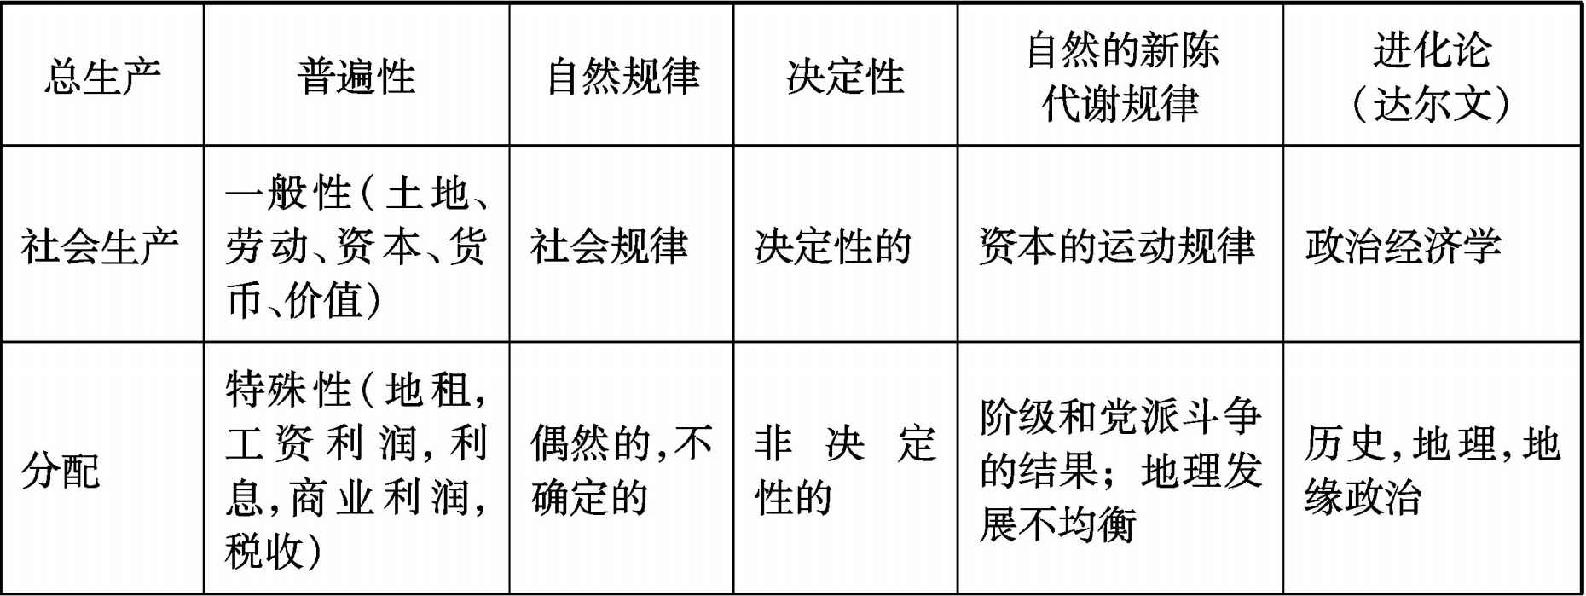
\includegraphics[scale=0.35]{david1.jpg}
\caption{马克思在《资本论》中采用的“弱三段论”分析框架}


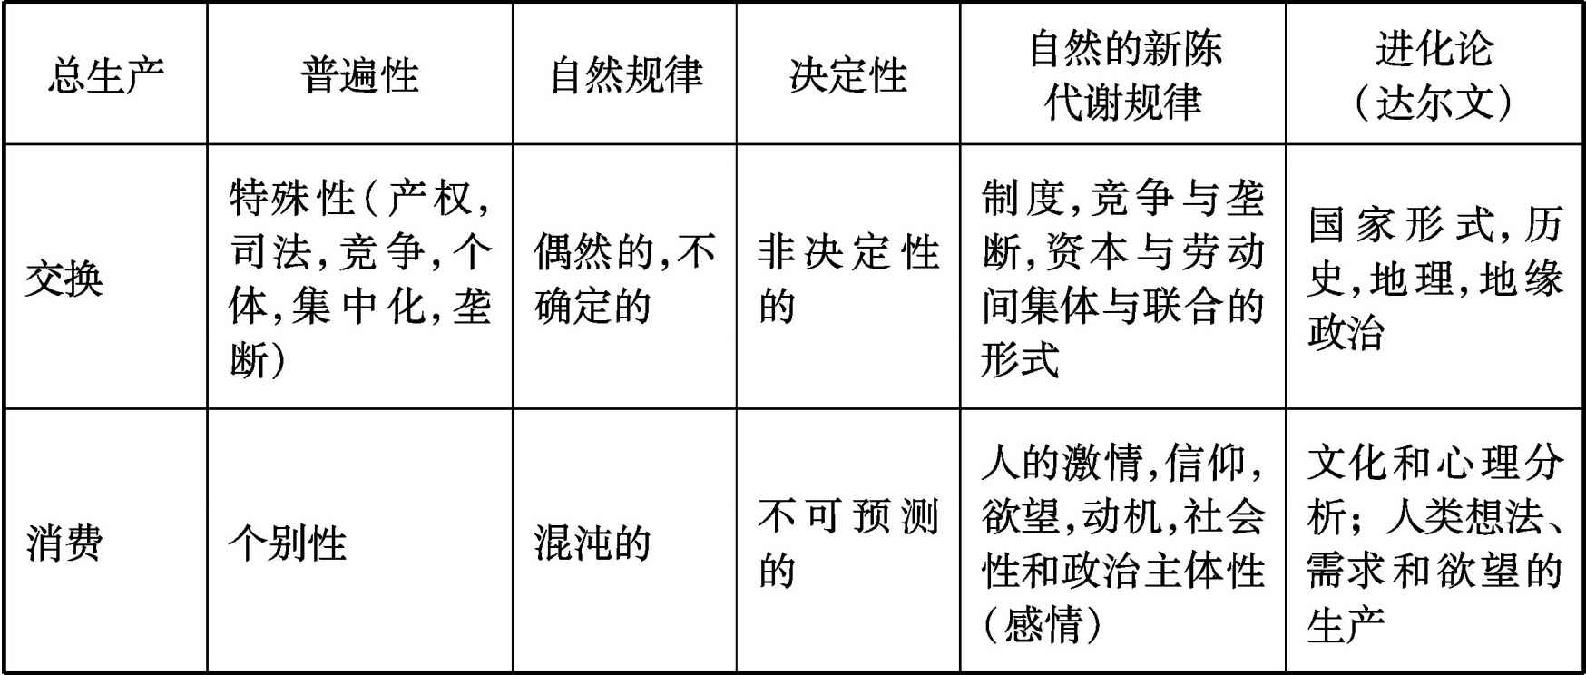
\includegraphics[scale=0.35]{david2.jpg}
\caption{续图1}
\end{figure}

尽管这个三段论“被公认为是一致的”,马克思说它还只是“肤浅的”。所以他拒绝了这个三段论,而是用辩证法研究了生产、分配、交换和消费怎样在构成资本主义生产方式的关系总体中结合起来。马克思对生产和消费、生产和分配、生产和交换的内在辩证关系进行了一系列讨论后得出了结论。生产、分配、交换和消费“构成一个总体的各个环节、一个统一体内部的差别\ldots{}\ldots{}不同要素之间存在着相互作用。每一个有机整体都是这样”。\pagescite[][37]{karlvol46a} 


马克思所想的资本主义生产方式的有机整体(总体)并不完全是黑格尔式的(尽管它来自于
对黑格尔概念的革命性改造,而非仅仅是简单地颠倒过来使用)。它的结构是生态系统的,
由葛兰西和列斐伏尔所说的不同时刻“总体”或德勒兹所说的不同时刻的“组合”的关系组成。马克思抱怨道:“对于一个黑格尔主义者来说,把生产和消费等同起来,是最简单不过的事。不仅社会主义美文学家这样做过,而且平庸的经济学家也这样做过。”\pagescite[][31]{karlvol46a} (Big Note)


读者也许期待马克思用辩证法和有机的理论来构建他的替代理论。但是从《资本论》的写作实践来看,即使他使用有机的思维和辩证的——关系性的分析来建构他的批判和探索另一种理论,很显然他最后还是遵循了古典政治经济学的三段论架构框架。他始终尽可能地贴近资产阶级关于生产一般的规律层次的概念,排除了具有“偶然性”和社会特殊性的分配和交换(直到在第三卷的最后部分才进行了讨论),至于混乱的消费的个别性当然更是如此。

在这里我要提出一点警告,这个排除有时是过分的(马克思应该做出说明)。(笔者注:马
克思对劳动力价值、在第三卷中“详细分析信用制度和它为自己所创造的工具(信用货币等),在我们的计划之外。在这里,只着重指出为说明资本主义生产方式一般的特征所必要的少数几点。”\pagescite[][350]{capital3} 


我最好的假设是,马克思根本的意图是以子之矛攻子之盾,用古典政治经济学自己的术语批判它本身。所以为了说明古典政治经济学的内在矛盾和不足,他不得不接受了这些术语的一般性质。因此如果资产阶级理论家事先假定了一个非强制的自由市场,那么马克思也需要这样做(就像他在第一卷第2章中所做的那样)。如果一般、特殊和个别之间的区别是资产阶级思维模式的基础,那么马克思也需要使用这个基础。这是我能给出的唯一答案,但还是不能完全让人满意,因为马克思接受了一些资产阶级的术语而拒绝了其他的。比如马克思在第一卷中没有涉及供给和需求或效用的问题(我们不久将看到他为什么这样做)。他从不对自己选择的逻辑进行解释。很明显他通篇都作出了这样的选择。

一般、特殊和个别这三个层次并不是故事的全部,还有第四个层次——普遍性——涉及与自然的
新陈代谢关系。马克思对古典政治经济学家把生产视作“包裹在独立于历史之外的永恒的自
然法则中”的做法表示了强烈反对。马克思反对把资本主义政治经济学“自然化”,从不放
弃任何抨击这种自然主义观点的机会(包括李嘉图学派和马尔萨斯学派认为利润率注定会下
降是因为自然资源的缺乏和地租上涨的观点)。马克思强调资本主义生产方式的一般性不能
用自然法则的普遍性解释。虽然马克思同意“资本主义生产”是规律般的一般性,他还是拒
绝以自然科学的方式将其理解为纯粹“自然”的东西。资本主义虽然是具有规律性的,但是
这些规律(包括那些关于私人财产关系的)是人类行为的产物。

为什么要赋予生产以优先权呢?马克思认为“生产既支配着与其他要素相对而言的生产自身,
也支配着其他要素。过程总是从生产重新开始”。这句奇怪的话是什么意思呢?\textbf{把
  支配自身的生产解释为产品和服务的物质生产,或是具体的劳动过程,甚至是商品的生产
  都是错误的。}非常不幸的是,这是个十分常见的误读,导致了对马克思认为社会关系、思
想、人类欲望等是由物质资料生产决定的说法的误解。这是生产主义和物质主义的误读,并
不是真正的马克思的历史唯物主义。(Big Note)


\textbf{在资本主义生产方式中占主导的生产是剩余价值的生产,剩余价值是社会性的,而
  不是物质性的关系。},在马克思宏伟的计划中,这意味着为他人生产剩余价值的社会需要
扭曲和支配了人的感觉器官通过劳动过程所能获得的解放的潜能。这个结果是对人类自身潜
在生产力和创造力的普遍异化。《政治经济学批判大纲》和《资本论》中一些最有说服力的
章节再三强调了这点。(笔者注:恩格斯致约·布洛赫(1890年9月21-22日)“根据唯物史
观,历史过程中的决定性因素归根到底是现实生活的生产和再生产。无论马克思或我都从来没
有肯定过比这更多的东西。如果有人在这里加以歪曲,说经济因素是唯一决定性的因素,那末
他就是把这个命题变成毫无内容的、抽象的、荒诞无稽的空话。”恩格斯同样强调了这点。
而经济基础决定上层建筑,上层建筑又反过来作用于经济基础是后来人对恩格斯这句话下面
部份的演绎,且过于决定论和片面化。)(Big Note)

简言之,通过资本循环进行的剩余价值的生产是规律般的资本主义生产方式的核心:没有剩余价值,就没有资本主义。这是马克思对古典政治经济学做出的根本性突破。马克思继续写道:

\begin{quotation}
交换和消费不能是起支配作用的东西,这是不言而喻的。分配,作为产品的分配,也是这样。而作为生产要素的分配,它本身就是生产的一个要素。因此,一定的生产决定一定的消费、分配、交换和这些不同要素相互间的一定关系。当然,生产就其单方面形式来说也决定于其他要素。\pagescite[][36-37]{karlvol46a} 

\end{quotation}

资本主义生产方式的“规律”事实上采取了以下形式:各种各样可能的、偶然的分配和交换
结构和多样化的消费体制在原则上都是可能的,只要它们不会过度限制或破坏规模不断扩大
的生产剩余价值的能力。\ldots{}\ldots{}从剩余价值生产的一般规律并不能直接推演出唯
一的分配模式、交换体系或特定的消费文化体制。但是——这是个很重要的“但
是”——它的可能性不是无限的。在任何时刻,包括与自然的关系,如果出现了过分地限
制或破坏剩余价值生产能力的情况,那要么资本将不复存在,要么总体关系必须作出全面调
整。这就是“决定”的含义。

供给和需求还有价格的波动对经济达到均衡状态很重要,但是均衡在哪里可以达到并不能用它们来解释。马克思在大多数情况下通过假设把这种扭曲排除在外,但有时因为系统的相关性他还是会把这些因素加入到思考中,比如在劳动价格问题上。

“竞争一般来说是资本贯彻自己的生产方式的手段”。竞争使资本的内在规律得到贯彻,使
这些规律对于个别资本成为强制规律。但是它并没有发明这些规律。竞争实现这些规
律”。\pagescite[][271]{karlvol46b}其他力量建立起资本运动的内在规律,竞争仅仅是执
行者和实施者,就像供给和需求那样。

\begin{quotation}
  资本主义生产的发展,使投入工业企业的资本有不断增长的必要,而竞争使资本主义生产
  方式的内在规律作为外在的强制规律支配着每一个资本家。竞争迫使他不断扩大自己的资
  本来维持自己的资本,而他扩大资本只能靠累进的积累。\pagescite[][683]{capital}

\end{quotation}

当垄断和寡头组织占据支配地位时,资本运动规律(甚至价值本身)会发生改变。这反映在20世纪60年代由保罗·巴兰、保罗·斯威齐还有法国共产党提出的(国家)垄断资本主义理论中。

但是,垄断阶段之后通常会进入另一个阶段,这时竞争的强制规律的恢复成为主要的政治关
切。20世纪70年代末资本主义世界的大部分国家普遍经历了这个过程。毕竟,这是新自由主
义的中心议程。资本家经常抱怨竞争是“破坏性的”,但是垄断很容易产生“滞胀”,就像
巴兰和斯威齐所说的那样。资本主义国家的政策经常试图在垄断(通过对经济“制高点”实
行国有化)和竞争(通过反兼并、反垄断立法,以及或情愿或不情愿地走向私有化和全球化
竞争)两者之间保持平衡。(Big Note)

操纵和调动人的欲望一直处在资本主义历史的中心,但马克思把它排除在了政治经济学之外,认为这属于历史研究的范畴。不过,它并非完全处于理论思考之外。(Big Big Note)


例如劳动者可以选择怎样花钱和用钱买什么,因此知道他们的想法、需求和欲望就变得非常重要。马克思认为,为了在不同的经济部门之间保持必要的均衡,资产阶级必须操纵大众消费,以使工人的消费相对于资本主义积累是“合理的”。资产阶级的博爱于是经常体现为教导劳动者的消费习惯,使之有利于积累。奢侈品和工资品之间的差别也变得很重要。(Big Big Note)

因此,马克思留给我们的一部分工作是对当代的消费主义找到比目前更好的解释。传统的政
治经济学研究的方法论在解释消费方面不太有效(马克思反对把太多消费的例子加入到政治
经济学领域中可能也是出于这个原因)。这同样适用于生产性消费——在商品生产的劳动过程
中用劳动消费原材料。控制劳动者在工作中的个性的困难已经被认识到了(尤其是在马里奥·特
隆蒂和安东尼奥·奈格里的作品中),正是这种个性蕴含着巨大的革命性潜力。

马克思认为消费是个别性而不是一般性也是因为这个道理。但是,马克思的历史著作的最终目的是把资本主义生产方式作为一个演进的有机整体来理解(与强调规律的政治经济学相反),因此任何对当代形势加以理解的尝试,都要求我们把消费、政治主体性和个体的审美、文化、政治偏好加入到研究框架中——作为政治经济学分析的基础和补充,而不是作为替代品。

在一般性方面的严格限制让马克思对资本的理解超越了他所在的时代的历史特殊性。这也是
为什么我们至今仍能阅读马克思著作的原因——即使是第二卷——而且还能够理解很多
他想要表达的内容。另一方面,很难将这个框架直接用于分析我们的现实状况,这也是我们
将要进行的工作。

\chapter{资本循环(第二卷 第1—3章)}

\begin{figure}
\centering
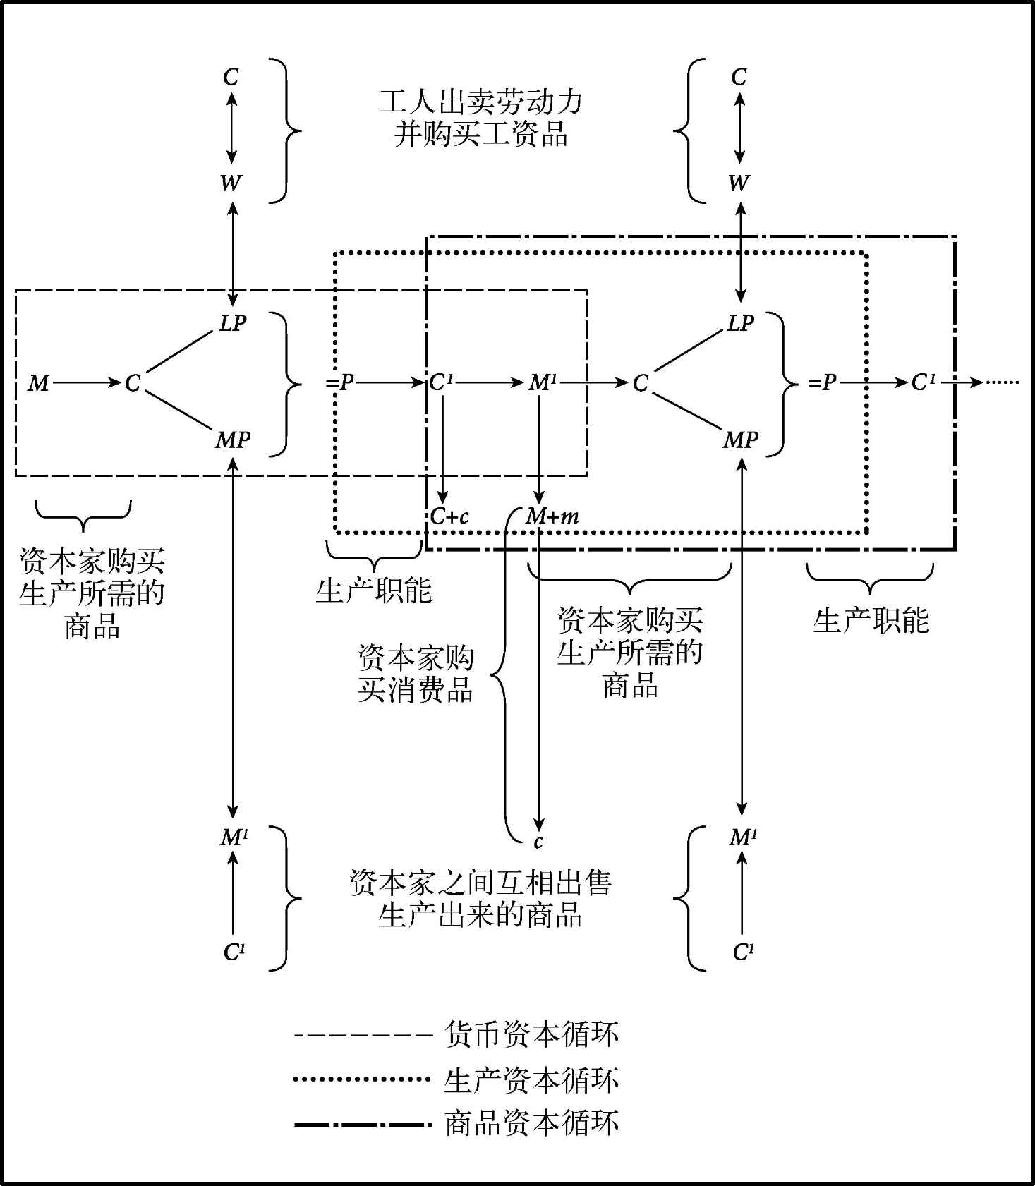
\includegraphics[scale=0.35]{david3.jpg}
\caption{产业资本循环的总公式,三个不同循环}
\end{figure}

在货币形态,资本可以像蝴蝶一样到处自由地“飞翔”;在商品形式上,资本就像毛虫一样,到处寻找想要、需要或是渴望得到它,有支付能力并最终消费它的人;作为劳动过程,资本植根于“生产的隐秘之处”(马克思在第一卷中提到),在这里,物质活动将自然要素转化为商品的生产。

资本在不同形态下进行的空间和地理运动的差异,对于理解我们统称为“全球化”的过程有
重要启发。

\begin{quotation}
  在生产危机和商业危机中称为货币危机的那一刻暴露得特别明显。这种货币危机只有在一
  个接一个的\textbf{支付的锁链}和抵消支付的人为制度获得充分发展的地方,才会发生。
  当这一机制整个被打乱的时候,不问其原因如何,\textbf{货币就会突然直接地从计算货
    币的纯粹观念形态转变成坚硬的货币}。这时,它是不能由平凡的商品来代替
  的。

  商品的使用价值变得毫无价值,而商品的价值在它自己的价值形式面前消失了。昨天,资
  产者还被繁荣所陶醉,怀着启蒙的骄傲,宣称货币是空虚的幻想。只有商品才是货币。今
  天,他们在世界市场上到处叫嚷:只有货币才是商品!他们的灵魂渴求货币这惟一的财富,
  就像鹿渴求清水一样。在危机时期,商品和它的价值形态(货币)之间的对立发展成绝对
  矛盾。\pagescite[][161-162]{capital} (Big Note)

  使劳动力的使用权归属于买者。而使用这种劳动力的界限,和劳动力本身价格的再生产所
  必需的劳动量的界限,又决不是一致的。资本关系所以会在生产过程中出现,只是因为这
  种关系在流通行为中,在买者和卖者相互对立的不同的基本经济条件中,在他们的阶级关
  系中本来就已经存在。不是由于货币的性质产生了这种关系;相反,\textbf{正是由于这
    种关系的存在,单纯的货币职能才能转化为资本职能。}\pagescite[][39]{capital2}

  要使资本能够形成并且能够支配生产,需要商业发展到一定的阶段,因此也需要商品流通
  从而商品生产发展到一定的阶段。……只有在资本主义生产的基础上,商品生产才表现为
  生产的标准的、占统治地位的性质。\pagescite[][40]{capital2} (Note)

  那些造成资本主义生产的基本条件,即雇佣工人阶级的存在的情况,也促使一切商品生产
  过渡到资本主义的商品生产。资本主义的商品生产越发展,它对主要是直接满足自己需要
  而只把多余产品转化成商品的每一种旧生产形式,就越发生破坏和解体的作用。\pagescite[][43]{capital2} 

  我们在重商主义体系的辩护人那里,发现了这样冗长的说教:资本家个人只应该和工人一
  样消费,资本家国家应该把它们的商品让给其他比较愚昧的国家去消费和进行消费过程,
  而相反地应该把生产消费当作自己的终生事业。这种说教在形式上和内容上往往使人想起
  教父们类似的禁欲诫条。\pagescite[][70]{capital2} (Big Note)

\end{quotation}
有一些人,例如凯文·菲利普斯,相信我们在过去十几年里经历了重商主义阶段,而美国担当的正是最愚昧的国家的角色(进行债务支撑的消费主义),中国人和德国人则以美国消费者为代价储蓄和积累了大量的贸易盈余。奥巴马当局在出席2010年秋季在首尔举行的G20峰会时,提议减少全球体系中的贸易不平衡,中国和德国是反对这个提议的主要国家。所以,某种形式的重商主义确实存在,而且状况良好——美国似乎仍然乐于担当最愚昧的国家的角色。(Big Note)

\begin{quotation}

  只要把这种形式(货币资本循环)不是当作循环形式的一种,而是当作惟一的循环形式,
  它的虚幻的性质以及与它相适应的虚幻的解释就会存在。但是,它本身已经指出其它的形
  式。\pagescite[][72]{capital2} 

  货币资本转化为生产资本,就是为生产商品而购买商品。只有消费是这种生产消费(剩余
  价值),它才进入资本本身的循环。…… 这样一种由剩余价值的生产所决定的用商品代替
  商品,和本来的产品交换(只是以货币为中介)完全不同。可是,经济学家们竟以此证明
  生产过剩是没有可能的。\pagescite[][87]{capital2} 

\end{quotation}

需要着重指出一点,如果工人将收入用来赌博(甚至是储蓄),而不是用来购买商品,那么循环过程的连续性就会遭到破坏。因此第二卷最后关注建立工人阶级的“合理消费”,将之作为稳定积累的条件的问题

\begin{quotation}
  商品的潮流一浪一浪涌来,最后终于发现,以前涌入的潮流只是表面上被消费吞没……以
  前涌入的商品还没有变成现金,支付期限却已经到来。商品持有者不得不宣告无力支付,
  或者为了支付不得不给价就卖。这种出售同需求的实际状况绝对无关。同它有关的,只
  是\textbf{支付的需求},只是把商品转化为货币的绝对必要。于是危机爆发
  了。\textbf{它不是表现在消费需求,即个人消费需求的直接缩减上,而是表现在资本对
    资本的交换,即资本再生产过程的缩减上。}\pagescite[][89]{capital2} (Big Big Note)

\end{quotation}

在个人消费领域表现出来的工人和资本家的有效需求不足,事实上可能是由于生产资料的购买和售卖的循环过程出现了问题。(Big Big Note)

关于工人阶级的有效需求和消费,马克思在第二卷中有两处看似非常矛盾的论述:
\begin{enumerate}
\item {\kaishu 资本主义生产方式中的矛盾:工人作为商品的买者,对于市场来说是重要的。
    但是作为他们的商品——劳动力——的卖者,资本主义社会的趋势是把它的价格限制在最低
    限度——还有一个矛盾:资本主义生产全力扩张的时期,通常就是生产过剩的时期;因为
    生产能力从来没有能使用到这个程度,以致它不仅能够生产更多的价值,而且还能把它
    实现。商品的出售,商品资本的实现,从而剩余价值的实现,不是受\textbf{一般社会
      的消费需求的限制},而是受\textbf{大多数人总是处于贫困状态、而且必然总是处于
      贫困状态的那种社会的消费需求的限制}。\pagescite[][350]{capital2} }

 
\item {\kaishu 认为危机是由于缺少有支付能力的消费或缺少有支付能力的消费者引起的,
    这纯粹是\textbf{同义反复}。除了需要救济的贫民的消费或“盗贼”的消费以外,资本
    主义制度只知道进行支付的消费。商品卖不出去,无非是找不到有支付能力的买者,也
    就是找不到消费者(因为购买商品归根结底是为了生产消费或个人消费)。但是,如果
    有人想使这个同义反复具有更深刻的论据的假象,\textbf{说什么工人阶级从他们自己
      的产品中得到的那一部分太小了,只要他们从中得到较大的部分,即提高他们的工资,
      弊端就可以消除},那么,我们只须提出,危机每一次都恰好有这样一个时期做准备,
    在这个时期,工资会普遍提高,工人阶级实际上也会从供消费用的那部分产品中得到较
    大的一份。按照这些具有健全而“简单”(!)的人类常识的骑士们的观点,这个时期
    反而把危机消除了。因此,看起来,资本主义生产包含着各种和善意或恶意无关的条件,
    这些条件只不过让工人阶级暂时享受一下相对的繁荣,而这种繁荣往往只是危机风暴的
    预兆。\pagescite[][456-457]{capital2} }
\end{enumerate}

第二个论述与第2章的精神更为一致,所以很明显,马克思认为从生产资本的角度展开的论述
具有更普遍的重要性。于是我们就面临一个难题:该追随哪个观点?我自己的想法是(你也
可以有自己的想法),这种情形可以出现,正如20世纪60年代末70年代初那样,劳动所得占
国民产出份额的上升,即便不是全球资本主义危机的根本原因,也至少是其先兆。但是,不
可能用这个观点来分析2007—2008年的经济崩溃。\textbf{工人阶级的分配份额,无论是过高
  还是过低,虽然有重要影响,但还不足以解释资本的危机倾向}。

\begin{quotation}
在P……P`中,P`所表示的,不是剩余价值被生产出来,而是生产出来的剩余价值已经资本
化,就是说,资本已经积累。\pagescite[][93]{capital2} (Big Big Note)

一个在资本循环之外完成的、为使剩余价值转化为实际执行职能的资本所进行的职能上确定
的预备阶段……只要它停留在贮藏状态中,它就还不是执行货币资本的职能,而是闲置的货
币资本;不是像前面所说的那种职能中断的货币资本,而是还不能执行职能的货币资本。\pagescite[][97]{capital2} 

\end{quotation}

在将特殊形式的价值和剩余价值转化成作为一般等价物的货币的困难之外,我们现在再加上
另一个困难:在市场中寻找必要的商品以\textbf{满足特定劳动过程中的生产性消费的需要}。
资本家必须依靠其他资本家生产自己所需的生产资料。因此,主要是在商品资本的循环中,
我们面临资本家之间特殊的相互关系和相互依赖的难题。随着第二卷内容的展开,越来越明
显的是,这种资本家之间的相互关系受到\textbf{充足供应(adequate supply)危机}的可
能性的困扰,更明显的问题可能是由有效需求不足引起的危机。

在生产率不变的情况下,规模扩大的再生产(撇开对外贸易)只有在剩余产品的待资本化的部分已经包含追加生产资本的物质要素时才能进行。\pagescite[][114]{capital2} 

\begin{quotation}
  正因为W′……W′ 循环在进行中要以另一个在W(=A+ Pm)形式上的产业资本为前
  提(并且Pm还包括各种其他资本,用我们的例子来说,包括机器、 煤炭、 润滑油等等),
  所以,这个循环本身就要求我们不仅把它看作循环的\textbf{一般}形式,即能够用来考察
  每一个\textbf{单个}产业资本 ( 第一次投资的场合除外) 的社会形式,因而不仅看作一
  切单个产业资本共有的运动形式,而且同时看作各单个资本的总和即资本家阶级
  的\textbf{总资本的运动形式},在这个运动中,每一个单个产业资本的运动,都只表现为
  一个部分运动,和其他部分运动交织在一起,并且受它们制
  约。\pagescite[][112]{capital2} (Big Big Note)

\end{quotation}
商品资本的循环很特别,它允许我们着眼于整体经济中的剩余价值和剩余产品(价值和使用
价值)的总的流动。……这种思维模式的先驱是魁奈。

在其他循环中,我们可以只关注个别的产业资本,而不必关心加总的情形。加总的情形只在商品资本的循环中出现。

\chapter{循环的三个公式和资本流动的连续性(第二卷 第4—6章)}

\begin{quotation}
  在一个不断回转的循环中,每一点都同时是出发点和复归点。……不仅每一个特殊的循环
  都把其他的循环作为前提( 包含在内),而且一种形式的循环的反复,已经包含着其他形式
  的循环的进行。 因此,全部区别表现为单纯形式上的区别,或者说,表现为单纯主观上
  的、 只对考察者才存在的区别。

资本在它的任何一种形式和任何一个阶段上的再生产都是连续进行的,就像这些形式的形态变化和依次经过这三个阶段是连续进行的一样。可见,在这里,总循环是资本的三个形式的现实的统一。\pagescite[][117]{capital2} 

\end{quotation}

这里强调的是资本在这三种循环运动中的连续性、继起性、并存性和流动性。问题的反面则是阻碍和可能的中断。“资本的循环过程是不断的中断,是离开一个阶段,进入下一个阶段;是抛弃一种形式,存在于另一种形式;其中每一个阶段不仅以另一个阶段为条件,而且同时排斥另一个阶段。”\pagescite[][118]{capital2} (Big Big Note)

“那些把价值的独立化看作是单纯抽象的人忘记了,产业资本的运动就是这种抽象的实
现”。\pagescite[][122]{capital2} “独立化”暗示了一个特别的问题。价值可能是一个
抽象概念,但是它却有真实的影响(或者用第一卷的话来说,价值是“幽灵般的对象性”)。
(Big Note)

\begin{quotation}
  如果社会资本的价值发生\textbf{价值革命},他个人的资本就可能受到这一革命的损害而
  归于灭亡,因为它已经不能适应这个价值运动的条件。价值革命越是尖锐,越是频繁,独
  立化的价值的那种自动的、以天然的自然过程的威力来发生作用的运动,就越是和资本家
  个人的先见和打算背道而驰,\textbf{正常的生产过程就越是屈服于不正常的投机,单个
    资本的存在就越是要冒巨大的风险。}因此,这些周期性的价值革命证实了它们似乎应该
  否定的东西,即证实了价值作为资本所经历的、通过自身的运动而保持和加强的独立化。(Big Big Note)

\end{quotation}

这完全可以算是对我们现在所谓的“去工业化”导致的资本贬值危险的理论再现。
从20世纪80年代起,一股巨大的工厂倒闭浪潮冲击了底特律、匹兹堡、巴尔的摩、谢菲尔德、
曼彻斯特、埃森、里尔和都灵等老工业城市。这种现象不只在发达资本主义国家出现,孟买
的传统纺织业区和中国北部的老工业基地同样遭受了猛烈的冲击和损失。所有集中于工业生
产的社区几乎都在一夜之间被摧毁了。比如谢菲尔德在20世纪80年代的三年时间内,失去了
大概六万个钢铁生产的工作岗位,到处是荒凉的景象。当人们寻找原因时,却被告知,这一
切都是由一股被称为“全球化”的神秘力量引起的。当工会和社会运动抗议并寻求遏止工作
和谋生手段流失的途径时,却被告知这种神秘的力量是无法避免和不可阻挡的。(Big Big Note)

更正式的表述就是:个别的资本家为了追求相对剩余价值而组织价值的生产,但这样做产生
的新的价值关系反过来会摧毁他们自己。资本不仅生产自身统治的手段,还生产毁灭自己的
手段。……但是他们不对资本主义制度感到愤怒,反而对外国生产者、移民者、投机者和其
他一些仅仅是资本运动的内在规律中秘密的、隐藏的当事人感到愤怒。(Big Big Note)

\begin{quotation}
  只有各种干扰在循环反复中被排除,过程才能够在事实上正常进行;\textbf{干扰越大,
    产业资本家就必须持有越是大量的货币资本},才有可能等到干扰被排除;因为随着资本
  主义生产的进展,每一个单个生产过程的规模会扩大,预付资本的\textbf{最低限量也会
    随之增加},所以除了其他情况外,又加上这个情况,使\textbf{产业资本家的职能越来
    越转化为各自独立或相互结合的大货币资本家的垄断}。\pagescite[][124]{capital2}(Big Big Note)

  (产业资本的循环)是和各种极其不同的社会生产方式的商品流通交错在一起的……不论
  商品是建立在奴隶制基础上的生产的产品,还是农民的产品(中国人,印度的佃农),还
  是公社的产品(荷属东印度),还是国家生产的产品(如在俄罗斯历史早期出现的以农奴
  制为基础的国家生产),还是半开化的狩猎民族的产品等等,它们都作为商品和货币,同
  表现产业资本的货币和商品相对立。\pagescite[][126]{capital2} 

  资本家以货币形式投入流通的价值,小于他从流通中取出的价值,这是因为他以商品形式
  投入流通的价值,大于他以商品形式从流通中取出的价值。既然他只是作为资本的人格化,
  只是作为产业资本家执行职能,他供给的商品价值,总是大于他需求的商品价值……资本
  家的供给和需求的差额越大,就是说,他所供给的商品价值越是超出他所需求的商品价值,
  资本家的资本增殖率就越大。他的目的,不在于使二者相抵,而是尽可能使它们不相抵,
  使他的供给超出他的需求。就单个资本家来说是如此,就资本家阶级来说也是如此。\pagescite[][133]{capital2} 

\end{quotation}

过剩资本的处置或吸收问题(卢森堡提法比较重要,马尔萨斯、卢森堡、马克思关于这方面
的论述也可参考上一卷的笔记):购买剩余价值的需求是从哪里来的呢?如果这只是寻找更
多货币的问题,那么在某处的某人(例如我们时代的联邦储备系统;对马克思来说是黄金生
产者,他随后考虑了他们潜在的作用)能简单地满足这个要求。\textbf{但是我们必须从价
  值而不是货币的范畴来解决这个问题。}如果剩余价值在交换中实现,那么我们必须解释最
终与剩余价值交换的等量价值是从何而来的。从理论上说,我们得回答这个问题,但是不能在资本主义范围外寻求答案(例如马克思在本章前面提到的需求和供给的非资本主义来源),也不能假设存在一个专门进行挥霍性消费的阶级。

对于马克思的看法,这里有一个可能的解释。在这一章的开头,他说“过程的所有前提都表
现为过程的结果,表现为过程本身所产生的前提。每一个因素都表现为出发点,经过点和复
归点”。\pagescite[][116]{capital2} 或者,像马克思一开始说的那样,前提(资本家的
有效需求)现在表现为结果(剩余价值的占有)。在简单再生产中这可能会起作用,但是,
由这些章节的主要观点可知,这个过程不太可能不受任何干扰和中断地顺利进行下去。

但是,如果资本家如此行事,那么他就成了“非资本家”,“他作为非资本家花掉的,不是
花在他作为资本家的职能上,而是花在他的私人需要或享受上”。马克思还说:“这个假定
等于假定资本主义生产不存在,从而假定产业资本家本身不存在。因为只要假定发挥作用的
动机是享受,而不是发财致富本身,资本主义就从根本上被废除了。”享受和发财致富的区
别似乎对马克思的推理很重要。说资本主义是建立在个人自身的享受欲望的基础上的,就违
背了马克思在第一卷第24章中论证的观点。在那里,他认为资本主义基于“为了生产而生产
和为了积累而积累”,是独立于资本家的个人欲望之外的。尽管总存在消费和享受的欲望与
追加投资的必要性相互冲突的“浮士德时刻”,但是竞争的强制规律迫使资本家无可奈何地
选择了后者。所以,把资本家假定成贪恋消费品的个体,并将其作为资本积累的驱动力,是
不充分的;假定资本家的驱动力是通过攫取货币占有更大的社会权力,也是不充分的(尽管
我们以后会看到,与这个动机有一定的关系)。资产阶级的历史任务就是不断地进行资本积
累。“在技术上也是不可能的。资本家不仅必须形成一个准备资本,以应付价格的变动并等
待买卖上最有利的行情;他必须积累资本,以扩大生产,并把技术进步合并到他的生产机体
中去”。\pagescite[][137]{capital2}

当部分剩余价值被再投资于扩大再生产时,上文提出的解决有效需求问题的办法就更不可行
了。资本家不仅要为购买和实现最初循环的剩余价值提供必要的资金,而且得寻找更多的资
源来实现再投资所生产的剩余价值。因此,问题将会一直存在。

我宁愿大略说出我对马克思论点的理解。资本家的消费分为两种类型:个人消费(必需品和奢侈品)和生产性消费。后者要求将初始资本收回,用于另一轮的剩余价值生产,并追加投资于扩大再生产,这意味着对更多的生产资料和额外雇佣的劳动力所需的消费资料的需求(假设没有劳动节约型的技术改进)。竞争的强制规律推动了扩大再生产(因此,重点是发财致富,而不是享乐)。所以,来源于\textbf{明天的}扩大生产的需求(加上资产阶级消费),为今天生产的过剩商品提供了市场。

实际上,需要用出售明天的产品得到的货币支付今天生产的剩余价值。资本家的供给和需求
间暂存的缺口只能在信用货币(马克思在第二卷中刻意回避这个问题)的帮助下填补。实际
上,资本家没必要向别人借钱。他们只需要打个欠条,先买后付——这种做法由来已久了。因
此,\textbf{资本积累和债务积累紧密相连,谁也离不开谁。}遏制债务进一步发展(像共和党
在2011年做的那样),实际上是一场终结资本主义的战斗。这就是为什么紧缩政策,如果无
限期执行的话,不仅会阻碍经济增长,而且最终将导致资本主义的崩溃。(Big Big Note)

马克思也指出,资本主义的商品生产必须按“生产一般”的方式进行,并且和 “非资本主义的生产过程”没有任何特殊的物理属性上的差异。

资本是生产——理解为\textbf{剩余价值的生产(不是物质生产)},它支配着分配、交换和消
费的所有环节,更重要的是,支配着生产的物质过程本身。\textbf{资本的再生产总是被理
  解为劳动和资本的阶级关系的再生产}(在第一卷第23章中解释得很清楚)。(Big Note)

在所谓的“部分无产阶级化”的情况下,全球劳动力中的很大一部分人拥有一些土地和其他
家族或血缘资源,当他们遭遇失业、生病或残疾时就会回到这种状况。例如,在当代中国就
是这种情况,很多社会再生产的成本都是由农村地区承担的。更为冷酷无情的是,美国的农
业综合企业就是以这种方式把社会再生产的成本转嫁到墨西哥身上的:雇用非法移民来从事
有致癌作用的杀虫剂的喷洒工作,直到他们病入膏肓,从而不得不返回墨西哥农村,在那里
接受照顾或者死去。

资本的特性存在于有利于创造剩余价值的生产中的阶级关系之中,其一般性存在于由货币、
生产和商品资本循环构成的产业资本的循环过程之中。

因此,认为在不对其他循环的运行进行根本变革的条件下,就可以在生产领域实现深刻变革
的想法只能是妄想。向社会主义或共产主义过渡,不仅需要通过激烈的斗争去消灭生产中的
阶级关系,还需要逆转或者重建其他循环,以表明货币化、商品化和劳务的交换是怎样实行
变革,为生产中的联合劳动提供支持的。(Big Big Note)

这个结论在这些漫长而往往自负的历史中找到了支持:尝试在非资本主义方式的基础上重新
改造资本主义生产,特别是在联合劳动的口号下。工人控制、自我管理、工人自治和合作工
厂的尝试(20世纪70年代在欧洲和2001年经济危机后在阿根廷兴起的那种)一直受到怀有敌
意的商人和金融资本的控制力的威胁,在某些情况下一度被摧毁了。工人控制和工人自治的
梦想,经常在货币和商品资本力量,以及规训它们的交换价值规律的岩石上撞得粉碎。价值
增殖从而榨取剩余价值的驱动力难以阻挡。显著的例子是1956年西班牙法西斯专政时期巴斯
克县的工人合作社蒙德拉贡,它之所以能长期存在,部分是因为它建立了属于自己的信用机
构和市场机制,从而在三个循环中贯彻了自己的政治主张。它继续存在并且繁荣发展着,其
两百家企业中的大部分仍把参与者的回报差距控制在3∶1(相比之下,美国公司是400∶1,
甚至更高)。有人批评蒙德拉贡越来越依赖外包合同,因此是通过剥削其他地区而生存)。(Note)

联合劳动形式面对的困难主要来自一直存在的资本主义的价值规律。就像我们之前看到的,
价值规律支配并常常摧毁个别资本。一旦进入由价值规律支配的世界,企业就得服从这些规
律的规训力量。远离这种规训力量即使不是不可能的,也是很困难的。为了生存,蒙德拉贡
和那些在阿根廷复兴的工厂不得不寻找与价值规律相妥协的方式。这使我们得出了一个至少
表面上令人气馁的一般性结论,马克思已经在他对资本贬值和去工业化的分析中使我们为这
个结论做好了准备:不废除资本的运动规律和支撑这些规律的价值规律的无形却客观的力量,
就不能废除生产中的劳资阶级关系。但是马克思经常被历史转变的协同演化理论所吸引。如
果我们在这里加入协同演化理论的轮廓,那么一种反资本主义斗争的策略就浮现出来了。尽
管劳动和资本的阶级关系处在资本定义的核心,它被深深的嵌入到了循环过程的其他方面之
中,以至于不废除或者取代它旁边的支撑物就很难消除它。尽管我们仍然相信联合劳动、工
人自治和自我管理的原则,也为尝试实行这样的生产和生活方式的漫长的斗争史感到光荣,
我们还是得面对社会变革的所有其他方面,它们是把全社会从资本的统治下解放出来所必需
的。

对于生产性和非生产性劳动之间的区分,在没有一个明确的核算上的解决方案时,我们面对的难题就是:如果既要保留马克思的直觉洞察力,又要承认实施这种区分的困难性(不可行性?),我们该怎样继续研究下去?

如果连续性是唯一的顾虑,那么我们就可以说,生产、流通和实现过程的所有劳动(也可以
延伸到用于劳动力再生产的家庭劳动)都是维持并再生产资本的总体劳动的一部分。换句话
说,我们可以认为所有参与产业资本循环的劳动者都算生产性工人。但是在马克思看来,这
将会粉饰和掩盖一些重要的东西。

反过来,我们可以推知,如果施加在这些扣除额(或者不能促进资本循环运动加速)上的权
力过大的话,危机可能会发生。如果所有权力都在货币资本家(金融家)和商业资本家(商
人)手里,那么它会对这部分资本最终依赖的价值生产造成什么样的影响呢?例如,2007年
后爆发的全球经济危机,可能是因为非生产性的资本和商品循环(例如高盛和沃尔玛)攫取
了过多的(正如我们将要看到的,绝大部分是虚拟的)利润,吸干了生产活动的能量;相反,
也可能是因为生产循环的状况严重恶化,刺激资本涌入了非生产性资本和商品循环中,通过
掠夺而不是生产来进行资本积累。(Big Note)

\begin{quotation}

显然,生产时间和劳动时间越吻合,在一定时期内一定生产资本的生产效率就越高,它的价值增殖就越大。因此,资本主义生产的趋势,是尽可能缩短生产时间超过劳动时间的部分。不过,资本的生产时间虽然可以和它的劳动时间不一致,但前者总是包含后者,而且超过的部分本身就是生产过程的条件。\pagescite[][141]{capital2} 

流通时间的延长和缩短,对于生产时间的缩短或延长,或者说,对于一定量资本作为生产资本执行职能的规模的缩小或扩大,起了一种消极限制作用。资本在流通中的形态变化越成为仅仅观念上的现象,也就是说,流通时间越等于零或近于零,资本的职能就越大,资本的生产效率就越高,它的自行增殖就越大。例如,假定有一个资本家按订货生产,因此他在提供产品时就得到支付,又假定支付给他的是他自己需要的生产资料,那么,流通时间就接近于零了。\pagescite[][142]{capital2} 

\end{quotation}
因此,生产资料供给的地理和空间条件给资本主义生产施加了限制,因为把生产资料运输到劳动进行的生产地点需要耗费时间。……为了获得生产所必需的使用价值,资本家要面对各种潜在的供给约束和成本。他们还得面对由其他资本,以及具有地缘政治雄心的国家权力所施加的约束。

\begin{quotation}
过程越是按社会的规模进行,越是失去纯粹个人的性质,作为对生产过程的监督和观念上的总括的簿记就越是必要;因此,簿记对资本主义生产,比对手工业和农民的分散生产更为必要,对公有生产,比对资本主义生产更为重要。\pagescite[][152]{capital2} 

\end{quotation}
表面上是流通的过程也可以创造一些价值。这种互相掺杂的情况使核算噩梦变得更糟:把商品放在容器中会增加它的价值,而它待在货栈里的时间则要从价值中扣除(例如,货栈的租金)。

我自己的结论是,放弃会计核算,转而集中于分析加速运动、库存费用管理等做法的实质影响。马克思已经说明,这些做法对于资本主义发展来说都是极端重要的。当我们把交通运输和通讯的问题,及其暗含的空间生产问题纳入进来时,这些问题就更加重要了。

商品在空间上的流通,即实际的移动,就是商品的运输。运输业一方面形成一个独立的生产部门,从而形成生产资本的一个特殊的投资领域。另一方面,它又具有如下的特征:它表现为生产过程在流通过程内的继续,并且为了流通过程而继续。\pagescite[][170]{capital2} 

\begin{quotation}
  \textbf{知识和技能的积累,社会智慧的一般生产力的积累,就同劳动相对立而被吸收在
    资本当中,从而表现为资本的属性,更明确些说,表现为固定资本的属性,}只要固定资
  本是作为真正的生产资料而加入生产过程。因此,机器体系表现为固定资本的最恰当的形
  式,而固定资本——就资本对自身的关系来看——则表现为资本一般的最适当的形
  式。\textbf{另一方面,就固定资本被束缚在自己一定的使用价值的存在中这一点来看,
    它是不符合资本的概念的,}因为作为价值来说,资本对采取任何特定的使用价值形式都
  是无所谓的,它可以把任何一种使用价值形式作为自己一视同仁的化身来加以采用或者抛
  弃。从这方面来看,从资本对外部的关系来看,流动资本同固定资本相比表现为资本的适
  当形式。\pagescite[][210]{karlvol46b}(Big Note)

\end{quotation}

我们已经多次看到,\textbf{连续性、流动性和加速}是资本流动的本质特性,但是现在我们
遇到一个范畴:固定资本的目的是促进流动,但是它本身是固定而不是流动的。

我认为矛盾是这样的:资本在一个时点创造了一整套适应其需要的景观,而在未来的某一时点,为了适应资本积累永恒的扩张的力量,会破坏它并重新建立一套新的景观。资本或者在别处,或者在旧的废墟上建立新的地理景观;留下的是去工业化的或废弃的景观,它们是孤立和破败的。这就是熊彼特所说的“创造性毁灭”。这一过程周期性地使资本循环和积累的地理景观发生贬值和变革——以惊天动地的方式。(Big Big Note)

原则上(尽管实际中并不总是这样),固定资本一直是永远对立的资本—劳动关系之外的一个常见的危机来源。危机在固定性不能适应扩张性的运动时发生。后者不得不打破已经固化的那部分资本所施加的限制。随着高度流动的货币资本流向别处,结果是大量固定资本的贬值。(1970年以来的去工业化留下了很多荒废的工厂、仓库和破败的基础设施——甚至衰退的城市,比如底特律)。(Big Big Note)

只被生产地消费,不能进入个人消费……在它完全损耗以前一直保持独立的形式。运输工具则例外。运输工具在它执行生产职能、从而停留在生产领域时产生的那种有用效果即场所变更,同时可以进入个人消费,例如旅客的个人消费。这时,旅客使用运输工具就像使用其他消费资料一样,也要支付报酬。\pagescite[][178]{capital2} 

我对这种例外情况很感兴趣,它意味着“场所变更”(从而,空间关系的生产)的有用性不仅适用于生产过程(原材料的移动),也适用于消费(人的移动)换句话说,“场所变更”的生产本身就是一种商品,不论谁使用它,也不论是为了什么目的(进一步的生产或者最终消费)。

\begin{quotation}
同一物品可以时而成为生产资本的组成部分,时而属于直接的消费基金。例如,一所房子,用作劳动场所,是生产资本的固定组成部分,用作住宅,就根本不是资本的形式,而只是一所住宅。在许多场合,同一些劳动资料,可以时而充当生产资料,时而充当消费资料。\pagescite[][227]{capital2} 

\end{quotation}
一个没有飞机起飞的机场是没有价值的。但是,没有机场的飞机也是没有价值的。注意,在
这个例子中很明显的是,可移动的固定资本形式(包括它们所携带的在市场上流通的商品资
本)在地理上的移动模式,受到另一些固定资本的增殖要求的限制——这些通常数额巨大的固
定资本被固定在了某个地方。不可移动的固定资本价值的收回,取决于运动中的资本对特定
地点的不可移动资本的使用。这产生了诸如城市间竞争的现象——将高度流动性的资本吸引并
保留在城市中(往往以对私人企业大量的公共补贴告终)。

\begin{quotation}
  可以利用的空间。有些建筑物可以加高几层;有些建筑物必须横向扩张,这就要有更多的
  地皮。在资本主义生产中,一方面有许多资财被\textbf{浪费}掉;另一方面,在企业逐渐
  扩大时,又有许多这种\textbf{不恰当的横向扩张(部分地说对劳动力有害)},因为一切
  都不是按照社会的\textbf{计划}进行的,而是取决于单个资本家从事经营活动的千差万别
  的环境、资财等等。由此就产生了生产力的巨大浪费。货币准备金(即再转化为货币的那
  部分固定资本)这样一部分一部分地再投入企业,在农业中实行起来最容易。在这里,有
  一定空间的生产场所,能够最大限度地逐渐地吸收资本。在进行自然再生产的地方也是这
  样,例如畜牧业。\pagescite[][193]{capital2}(Big Note)

  再从另一方面看,\textbf{固定资本的发展也表明一般财富发展的程度,或者说资本发展
    的程度。}直接以使用价值为目的的生产,以及直接以交换价值为目的的生产,其对象都
  是供消费用的产品本身,生产固定资本的那部分生产既不生产直接的消费品,也不生产直
  接的交换价值,至少\textbf{不生产可以直接实现的交换价值}。因此,越来越大的一部分
  生产时间耗费在生产资料的生产上,这种情况取决于已经达到的生产率水平,取决于用一
  部分生产时间就足以满足直接生产的需要。这就要求社会能够等待;能够把相当大一部分
  已经创造出来的财富从直接的享受中,也从以直接享受为目的的生产中抽出来,以便(在
  物质生产过程本身内部)把这一部分财富用到非直接生产的劳动上去。这就要求已经达到
  的生产率和相对的富裕程度都有高度水平,而且这种高度水平是同流动资本转变为固定资
  本成正比的。正如相对剩余劳动的大小取决于必要劳动的生产率一样,用于生产固定资本
  的劳动时间——活劳动时间和物化劳动时间——的大小也取决于直接用于生产产品的劳动时间
  的生产率。\textbf{过剩人口(从这个观点来看),以及过剩生产,是达到这种情况的条
    件。}这就是说,用在直接生产上的时间所取得的成果相对说来必定很大,超出了这些生
  产部门所使用的资本的再生产的直接需要。固定资本带来的直接成果越少,越少参与直接
  生产过程,这种相对的过剩人口和过剩生产就应该越多;因而,修建铁路、运河、自来水、
  电报等场合,同制造直接用于直接生产过程的机器的场合相比,过剩人口和过剩生产就应
  该多些。由此(我们以后将回过头来谈这一点)就产生出——通过现代工业中经常生产过剩
  和经常生产不足的形式——这样一种状态:流动资本向固定资本的转化有时过多有时过少,
  这种不平衡状态经常波动和痉挛。\pagescite[][220-221]{karlvol46b} 

\end{quotation}
固定资本投资——包括初始购买和补偿——的“团块结构”(lumpiness)是一个显著的特点。它在货币方面的影响是决定了在特定时刻有多少货币资本应该从流通中撤出或回归流通:

此外,在再生产一部分一部分地进行,使已经损坏的部分在较短时间内换新的地方,在这种补偿能够实行之前,必须根据生产部门的特殊性质,事先积累一笔或大或小的货币。为了这个目的,不是拥有随便一个货币额就行,而是必须拥有一定数量的货币额。\pagescite[][202]{capital2} 

\begin{quotation}
  生产资料的不断变革——这种变革也随着资本主义生产方式的发展而不断加快——又使它缩短。
  因此,随着资本主义生产方式的发展,生产资料的变换也加快了,它们因\textbf{无形损
    耗}而远在有形寿命终结之前就要不断补偿的必要性也增加了……这种由一些互相连结的
  周转组成的长达若干年的周期(资本被它的固定组成部分束缚住这种周期之内),为周期
  性的危机造成了\textbf{物质基础}。在周期性的危机中,营业要依次通过松弛、中等活跃、
  急剧上升和危机这几个时期。虽然资本投入的那段期间是极不相同和极不一致的,但危机
  总是大规模新投资的起点。因此,就整个社会考察,危机又或多或少地是下一个周转周期
  的新的物质基础。\pagescite[][206-207]{capital2}

\end{quotation}
加速折旧引起了现有固定资本的贬值,它的价值还没有通过商品的生产和销售而全部回流。
如果这种情况大规模地发生,显然会引发危机。正如马克思在第一卷中所说的,它对工人的
影响就是以换班和夜间工作的形式来劳动,以在无形损耗还没有冲击自己时就尽可能快地收
回固定资本的价值。但是第二卷一点也没有强调“无形损耗”或者其他社会力量(比如那些
使固定资本陷入困境的位置变化)导致的固定资本大规模贬值的普遍意义。《政治经济学批
判大纲》从历史和理论的角度提到了这一问题。所以我们要靠自己来探索这些意义。




马克思说,普遍的危机(显然,资本遭受了价值损失)也许是更新、补偿现存的固定资本的
好时机。这个观点需要进一步的论述。危机中,很多现存的固定资本处于闲置、贬值的状态
(资本利用率非常低),所以有货币贮藏的资本家或许就会抛弃现存设备来进行更新(尤其
是因为新固定资本的花费比较低)。在公共政策领域的一个近期的实例是由联邦政府
在2008年启动的所谓“旧车换现金”计划。消费者在旧车还没废弃时被给予现金,让他们买
新车、弃旧车。这样做的目标是活跃汽车市场,促进汽车产业的繁荣。对加速折旧的税收减
免是另外一个影响固定资本的更新和再投资的公共政策因素。20世纪80年代罗纳德·里根总统
在位时实行过。这是对大量现存的和新的固定资本进行加速折旧的公共补贴。事实上,这实
际上补贴了资本向美国南部和西部的运动以及东北部和中西部的去工业化。当然,这样做是
否具有更普遍的“有效性”,取决于新的技术可能性和区位可能性的存在。在美
国,20世纪30年代是技术和制度更新在危机条件下发生的显著时期,结果形成了一个完全不
同的固定资本投资模式(以汽车、电气化以及加州的开发为基础),它在二战后为美国带来
了繁荣。它“也是下一个周转周期的新的物质基础”。在当前萧条的情况下,是否存在相似
的固定资本投资环境的重组过程呢?如果存在,那在哪里?中国吗?马克思的相关理论值得
我们进一步的研究。

马克思危机形成和解决理论的这些方面的普遍意义,很少出现在马克思主义的文献中,尽管
有很多相关历史证据:商业周期与新技术浪潮,商业周期与大规模的“无形损耗”浪潮,都
以马克思概述的方式出现。生产能力利用率(主要是固定资本)被看做是经济健康的一个重
要指标。人们只要看看中国应对2008—2009年危机时的大规模固定资本投资,就可以明白这些
关系是如何重要。另一方面,我们可以看到下面这点是多么必要,“必须不断地有超额生产,
也就是说,生产规模必须大于单纯补偿和再生产现有财富所必要的规模——完全撇开人口的增
长不说——以便掌握一批生产资料,来弥补偶然事件和自然力所造成的异乎寻常的破
坏”。\pagescite[][198]{capital2} 尽管马克思这里主要考虑的是地震、海啸的影响,但
没有任何理由不将这个见解扩展到分析中国2009年经历的出口市场萎缩的情况。中国有大量
的剩余资本(就像英国从17世纪到19世纪末那样),所以不需要紧缩(如罗斯托和美国现今
的共和党所鼓吹的那样)就能为固定资本的大规模投资浪潮提供资金。然而,就像马克思如
此有预见性地指出的那样,这里也有“要依次通过松弛、中等活跃、急剧上升和危机这几个
时期”的周期性危机的“物质基础”。事实上,在资本主义生产方式的中心领域,各式各样
固定资本(包括固定在土地上的大量基础设施)的“无形损耗”能够也确实周期性地通过无
数种方式演变成严重的破坏和危机(尤其是资产价值)。马克思指出了这种一般的可能性,
但没有深入阐述,这在我看来是个遗憾。马克思提供了一些有建设性的想法,也给我们留下
了大量要做的工作。

“马克思经常为了方便把社会必要劳动等同于凝结劳动,但是后者并不包含作为一种社会关系的价值的所有方面。价值,我们回想一下,‘只存在于某种使用价值中’,所以,‘使用价值丧失,价值也就丧失’。这是因为‘商品在能够作为价值实现以前,必须证明自己是使用价值’。因此,‘如果物没有用,那么其中包含的劳动也就没有用,不能算作劳动,因此不形成价值’。”

我认为“价值不是一个用来描述变化着的世界的固定标准,而是一种社会关系,其核心体现了矛盾与不确定性。因此,在马克思的价值概念和固定资本流通的‘独特性’之间不存在什么矛盾。矛盾内化于价值本身的概念之中”。(Big Big Note)














%%% Local Variables:
%%% mode: latex
%%% TeX-master: "../main"
%%% End:
